\setcounter{section}{0}
\section{Lý thuyết}
\subsection{Biến dạng kéo và biến dạng nén}
Khi không có ngoại lực tác dụng, vật rắn có kích thước và hình dạng xác định. Khi có ngoại lực tác dụng, vật rắn thay đổi hình dạng và kích thước, ta nói vật rắn bị biến dạng.

\begin{minipage}{0.6\textwidth}
	\subsubsection{Biến dạng kéo}
	Dấu hiệu: Kích thước của vật theo phương tác dụng của lực tăng lên so với kích thước tự nhiên của nó.
	\subsubsection{Biến dạng nén}
	Dấu hiệu: Kích thước của vật theo phương tác dụng của lực giảm xuống so với kích thước tự nhiên của nó.
\end{minipage}
\begin{minipage}{0.4\textwidth}
	\begin{center}
		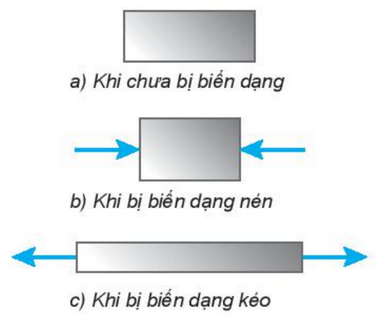
\includegraphics[scale=0.6]{../figs/G10-028-1}
	\end{center}
\end{minipage}
\subsection{Biến dạng đàn hồi}
Khi không còn tác dụng của ngoại lực, nếu vật rắn lấy lại được kích thước và hình dạng ban đầu thì biến dạng của vật là biến dạng đàn hồi.

Giới hạn mà trong đó vật rắn còn giữ được tính đàn hồi được gọi là giới hạn đàn hồi của vật rắn.

\subsection{Các đặc tính của lò xo}
Các loại lò xo đều có tính đàn hồi. Lò xo bị biến dạng kéo hoặc biến dạng nén tùy thuộc vào chiều của lực đặt vào hai đầu lò xo.

\begin{minipage}{0.6\textwidth}
	Độ biến dạng của lò xo (kí hiệu: $\Delta l$) là hiệu số giữa chiều dài khi bị biến dạng và chiều dài tự nhiên của lò xo.
	\begin{itemize}
		\item Khi lò xo biến dạng nén: độ biến dạng của lò xo âm, độ lớn của độ biến dạng được gọi là độ nén.
		\item Khi lò xo biến dạng kéo: độ biến dạng của lò xo dương và được gọi là độ dãn.
	\end{itemize}
	
	
	Khi hai lò xo chịu tác dụng bởi hai lực kéo/nén có độ lớn bằng nhau và đang bị biến dạng đàn hồi, lò xo có độ cứng (kí hiệu: $k$) lớn hơn sẽ bị biến dạng ít hơn.
\end{minipage}
\begin{minipage}{0.4\textwidth}
	\begin{center}
		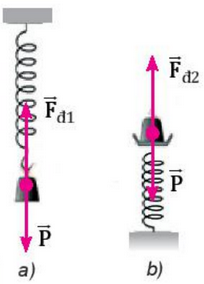
\includegraphics[scale=0.8]{../figs/G10-028-2}
	\end{center}
\end{minipage}

\subsection{Định luật Hooke}
\begin{minipage}{0.6\textwidth}
	
	Khi lò xo bị biến dạng, trong lò xo xuất hiện lực đàn hồi có xu hướng chống lại sự biến dạng. 			
	
	Trong giới hạn đàn hồi, độ lớn của lực đàn hồi của lò xo tỉ lệ thuận với độ biến dạng của lò xo.
	\begin{equation*}
		F= k \cdot |\Delta l|.
	\end{equation*}
	
	Trong đó:
	\begin{itemize}
		\item $k$ là độ cứng của lò xo (N/m). Hệ số $k$ càng lớn thì lò xo càng ít bị biến dạng. Độ cứng của lò xo phụ thuộc vào chất thép dùng làm lò xo, đường kính của vòng xoắn và tiết diện
		dây.
		\item $|\Delta l|=|l-l_0|$ là độ biến dạng của lò xo (m).
		\item $F$ là lực đàn hồi của lò xo (N).
	\end{itemize}
\end{minipage}
\begin{minipage}{0.4\textwidth}
	\begin{center}
		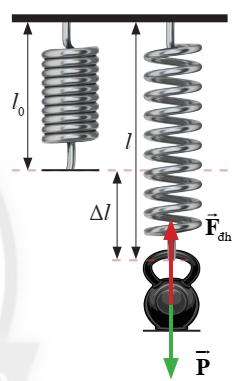
\includegraphics[scale=0.3]{../figs/G10-028-5}
	\end{center}
	
\end{minipage}
\subsection{Ứng dụng định luật Hooke}
\begin{minipage}{0.6\textwidth}
	Cân đồng hồ (hay còn gọi là cân đồng hồ lò xo) là loại cân được sử dụng nhiều trong đời sống. Cân đồng hồ lò xo bao gồm loại để bàn và loại có móc treo.
	
	Cân hoạt động dựa trên sự biến dạng của lò xo, tạo trạng thái cân bằng khi lò xo chịu tác dụng nén (cân đĩa) hoặc kéo (cân móc treo). Trên cân có bộ phận chuyển đổi chuyển động thẳng (do kéo  hoặc nén) của lò xo sang chuyển động xoay tròn của kim chỉ thị và hiển thị kết quả đo trên mặt số của đồng hồ.
\end{minipage}
\begin{minipage}{0.4\textwidth}
	\begin{center}
		
\includegraphics[scale=0.5]{../figs/G10-028-3}
	\end{center}
\end{minipage}

\section{Mục tiêu bài học - Ví dụ minh họa}
\begin{dang}{Nêu khái niệm biến dạng đàn hồi, biến dạng kéo và biến dạng nén}
	\viduii{1}{Kích thước và hình dạng của vật khi biến dạng kéo và biến dạng nén khác nhau như thế nào?
	}
	{	\begin{center}
			\textbf{Hướng dẫn giải}
		\end{center}
		
		\begin{itemize}
			\item Biến dạng kéo: Kích thước của vật theo phương tác dụng của lực tăng lên so với kích thước tự nhiên của nó.
			
			\item Biến dạng nén: Kích thước của vật theo phương tác dụng của lực giảm xuống so với kích thước tự nhiên của nó.
		\end{itemize}
	}
	\viduii{1}{Trong thí nghiệm với lò xo và vòng dây cao su, nếu lực kéo quá lớn thì khi thôi tác dụng lực, chúng có trở về hình dạng, kích thước ban đầu được không?
	}
	{	\begin{center}
			\textbf{Hướng dẫn giải}
		\end{center}
		
		Khi tăng cường độ lực tác dụng, độ giãn của lò xo và vòng dây cao su tăng. Tuy nhiên, khi tăng giá trị lực vượt quá một giới hạn nào đó thì khi dừng tác dụng lực, lò xo sẽ không thể chiều dài ban đầu nữa, hoặc vòng dây cao su sẽ bị đứt. Giá trị giới hạn này được gọi là giới hạn đàn hồi.
	}
	\viduii{2}{Tìm hiểu và giải thích tại sao ở Nhật Bản, nhiều tòa nhà cao tầng được xây dựng với các lò xo ở dưới móng cọc.
	}
	{	\begin{center}
			\textbf{Hướng dẫn giải}
		\end{center}
		
		Ở Nhật Bản, các tòa nhà khi được xây dựng đều phải tuân theo những tiêu chuẩn chống động đất rất khắt khe. Một trong số đó là việc có các lò xo ở dưới móng cọc. Mục đích của việc này là để lò xo hấp thụ xung lực từ các chấn động và giảm xóc cho tòa nhà.
	}
\end{dang}
\begin{dang}{Nhận biết đặc điểm của lực đàn hồi của lò xo. Ghi nhớ định luật Húc}
	\viduii{1}{Lực đàn hồi xuất hiện tỉ lệ với độ biến dạng khi 
		\begin{mcq}
			\item một vật bị biến dạng dẻo.
			\item một vật biến dạng đàn hồi.
			\item một vật bị biến dạng.	
			\item ta ấn ngón tay vào một viên đất nặn.
		\end{mcq}
	}
	{	\begin{center}
			\textbf{Hướng dẫn giải}
		\end{center}
		
		Lực đàn hồi xuất hiện tỉ lệ với độ biến dạng khi một vật biến dạng đàn hồi.
		
		\textbf{Đáp án: B}.
	}
	\viduii{1}{Điều nào sau đây là \textbf{sai}?
		\begin{mcq}
			\item Độ cứng của lò xo cũng được gọi là hệ số đàn hồi của lò xo.
			\item Lò xo có độ cứng càng nhỏ càng khó biến dạng.
			\item Độ cứng cho biết sự phụ thuộc tỉ lệ của độ biến dạng của lò xo vào lực gây ra sự biến dạng đó.
			\item Độ cứng phụ thuộc hình dạng, kích thước lò xo và chất liệu làm lò xo.
		\end{mcq}
	}
	{	\begin{center}
			\textbf{Hướng dẫn giải}
		\end{center}
		
		Lò xo có độ cứng càng lớn càng khó biến dạng.
		
		\textbf{Đáp án: B}.
	}
\end{dang}
\begin{dang}{Tính độ biến dạng của lò xo và các đại lượng trong định luật Húc}
	\viduii{2}{Một quả cân có khối lượng $m = \SI{100}{g}$ treo vào đầu dưới của một lò xo nhẹ, đầu kia của lò xo gắn trên giá treo. Cho $g= \SI{10}{m/s^2}$. Khi vật cân bằng thì lực của lò xo tác dụng lên vật là bao nhiêu?
	}
	{	\begin{center}
			\textbf{Hướng dẫn giải}
		\end{center}
		
		\begin{itemize}
			\item Vật chịu tác dụng của trọng lực $\vec{P}$ và lực đàn hồi $\vec{F}_{\text{đh}}$.
			\item Khi vật nằm cân bằng
			\begin{equation*}
				F_{\text{đh}} = P = mg =\SI{1}{N}.
			\end{equation*}
		\end{itemize}
	}
	
	\viduii{3}{Một lò xo có chiều dài tự nhiên là $\SI{30}{cm}$, khi bị nén lò xo dài $\SI{24}{cm}$ và lực đàn hồi của nó bằng $\SI{5}{N}$. Hỏi khi lực đàn hồi bị nén bằng lực  $\SI{10}{N}$ thì chiều dài của nó bằng bao nhiêu?
	}
	{	\begin{center}
			\textbf{Hướng dẫn giải}
		\end{center}
		
		Độ biến dạng của lò xo khi bị nén lúc đầu 
		\begin{equation*}
			\Delta l = l_0 - l = \SI{6}{cm}.
		\end{equation*}
		Độ cứng của lò xo
		\begin{equation*}
			k = \dfrac{F}{\Delta l} = \dfrac{250}{3}\ \text{N/m}.
		\end{equation*}
		Độ biến dạng của lò xo khi bị nén với lực \SI{10}{\newton}
		\begin{equation*}
			\Delta l' =\dfrac{F'}{k} = \SI{0,12}{cm}.
		\end{equation*}
		Chiều dài của lò xo lúc này
		\begin{equation*}
			l=l_0 -\Delta l = \SI{18}{cm}.
		\end{equation*} 
		
	}
	
	
	\viduii{3}{Một lò xo có chiều dài tự nhiên bằng $\SI{20}{cm}$ được treo thẳng đứng vào một điểm cố định. Khi treo vào đầu còn lại một vật có khối lượng $\SI{500}{g}$, lò xo có chiều dài $\SI{22}{cm}$ khi vật ở vị trí cân bằng. Lấy $g=\SI{9.8}{m/s^2}$.
		\begin{enumerate}[label=\alph*)]
			\item Tính độ cứng của lò xo.
			\item Để giữ vật nặng cố định tại vị trí lò xo có chiều dài bằng $\SI{19}{cm}$, cần tác dụng một lực nâng vào vật theo phương thẳng đứng có độ lớn bằng bao nhiêu?
		\end{enumerate}
	}
	{	\begin{center}
			\textbf{Hướng dẫn giải}
		\end{center}
		
		\begin{enumerate}[label=\alph*)]
			\item Tính độ cứng của lò xo.
			\begin{center}
				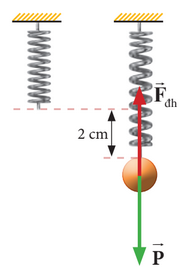
\includegraphics[scale=0.6]{../figs/G10-028-4}
			\end{center}
			
			Độ dãn của lò xo khi vật ở vị trí cân bằng:
			$$\Delta l = l - l_0 = \SI{22}{\centi\meter} - \SI{20}{\centi\meter} = \SI{2}{\centi\meter}=\SI{0.02}{\meter}.$$
			Khi này, lực đàn hồi của lò xo cân bằng với trọng lực của vật như phân tích lực trong hình bên:
			$$F_\text{đh} = m g = \SI{0.5}{\kilogram} \cdot \SI{9.8}{\meter/\second^2} = \SI{4.9}{N}$$
			Vậy độ cứng của lò xo:
			$$k=\dfrac{F}{\Delta l} = \dfrac{\SI{4.9}{\newton}}{\SI{0.02}{\meter}} = \SI{245}{N/m}$$
			
			\item Tại vị trí lò xo có chiều dài bằng $\SI{19}{cm}$, có ba lực tác dụng vào vật theo phương thẳng đứng: trọng lực có chiều hướng xuống; lực đàn hồi của lò xo lúc này có chiều hướng xuống vì lò xo bị nén so với chiều dài tự nhiên và lực nâng hướng lên.
			
			Khi này, lực đàn hồi có độ lớn:
			$$F_\text{đh} = k |\Delta l| = \SI{245}{\newton/\meter} \cdot |\SI{0.19}{\meter} - \SI{0.2}{\meter}| = \SI{2.45}{\newton}$$
			
			Do vật đứng yên nên lực tổng hợp tác dụng vào vật triệt tiêu, suy ra lực nâng của tay có độ lớn:
			$$F=m  g + F_\text{đh} =\SI{0.5}{\kilogram}\cdot\SI{9.8}{\meter/\second^2} + \SI{2.45}{\newton} = \SI{7.35}{\newton}$$
		\end{enumerate}
		
		\begin{center}
			\textbf{Câu hỏi tương tự}
		\end{center}
		
		Một lò xo bố trí theo phương thẳng đứng và có gắn vật nặng khối lượng $\SI{200}{g}$. Khi vật treo ở dưới thì lò xo dài $\SI{17}{cm}$, khi vật đặt ở trên thì lò xo dài $\SI{13}{cm}$. Lấy $g=\SI{10}{m/s^2}$ và bỏ qua trọng lượng của móc treo, giá đỡ vật nặng. Tính độ cứng của lò xo.
		
		\textbf{Đáp án:} $k=\SI{100}{N/m}$.
	}
\end{dang}
\section{Trắc nghiệm}
\begin{enumerate}[label=\bfseries Câu \arabic*:]
	\item \mkstar{2}
	
	
	{
		Khi nói về lực đàn hồi của lò xo, phát biểu nào sau đây \textbf{sai?}
		\begin{mcq}
			\item Lực đàn hồi luôn có chiều ngược với chiều biến dạng của lò xo.
			\item Trong giới hạn đàn hồi, lực đàn hồi luôn tỉ lệ thuận với độ biến dạng.
			\item Khi lò xo bị dãn, lực đàn hồi có phương dọc theo trục lò xo.
			\item Lò xo luôn lấy lại được hình dạng ban đầu khi thôi tác dụng lực.
		\end{mcq}
	}
	
	\hideall
	{	
		\textbf{Đáp án: D.}
		
		Lò xo chỉ lấy lại được hình dạng ban đầu khi bị biến dạng trong giới hạn đàn hồi.
	}
	\item \mkstar{2}
	
	
	{
		Một vật có khối lượng $\SI{200}{g}$ được treo vào một lò xo thẳng đứng thì chiều dài của lò xo là $\SI{20}{cm}$. Biết khi chưa treo vật thì lò xo dài $\SI{18}{cm}$. Lấy $g=\SI{10}{m/s^2}$. Độ cứng của lò xo này là
		\begin{mcq}(4)
			\item $\SI{200}{N/m}$.
			\item $\SI{150}{N/m}$.
			\item $\SI{100}{N/m}$.
			\item $\SI{50}{N/m}$.
		\end{mcq}
	}
	
	\hideall
	{	
		\textbf{Đáp án: C.}
		
		Khi lò xo treo thẳng đứng thì
		$$k|\Delta l| = mg \Rightarrow k =\dfrac{mg}{\Delta l} = \SI{100}{N/m}$$
	}
	\item \mkstar{2}
	
	
	{
		Hai lò xo A và B có chiều dài tự nhiên bằng nhau. Độ cứng của lò xo A là $\SI{100}{N/m}$. Khi kéo hai lò xo với cùng lực $F$ thì lò xo A dãn $\SI{2}{cm}$, lò xo B dãn $\SI{1}{cm}$. Độ cứng của lò xo B là
		\begin{mcq}(4)
			\item $\SI{200}{N/m}$.
			\item $\SI{150}{N/m}$.
			\item $\SI{100}{N/m}$.
			\item $\SI{50}{N/m}$.
		\end{mcq}
	}
	
	\hideall
	{	
		\textbf{Đáp án: A.}
		
		Lập tỉ lệ:
		$$\dfrac{k_\text A}{k_\text B} = \dfrac{|\Delta l_\text B|}{|\Delta l_\text A|} \Rightarrow k_\text{B} = \SI{200}{N/m}$$
	}
	
	\item \mkstar{2}
	
	
	{
		Một lò xo nằm ngang có chiều dài tự nhiên là $\SI{40}{cm}$, khi bị nén lò xo dài $\SI{35}{cm}$ và lực đàn hồi khi đó bằng $\SI{2}{N}$. Khi lực đàn hồi của lò xo bị nén là $\SI{5}{N}$ thì lò xo có chiều dài
		\begin{mcq}(4)
			\item $\SI{35}{cm}$.
			\item $\SI{32.5}{cm}$.
			\item $\SI{25}{cm}$.
			\item $\SI{27.5}{cm}$.
		\end{mcq}
	}
	
	\hideall
	{	
		\textbf{Đáp án: D.}	
		
		Lập tỉ số:
		$$\dfrac{F_\text{đh 1}}{F_\text{đh 2}} = \dfrac{|\Delta l_1|}{|\Delta l_2|} \Rightarrow |\Delta l_2| = \SI{12.5}{cm}$$
		
		Vậy $l_2 = \SI{27.5}{cm}$.
	}
	\item \mkstar{3}
	
	
	{
		Một lò xo đầu trên gắn cố định. Nếu treo vật nặng khối lượng $\SI{600}{g}$ vào một đầu thì lò xo có chiều dài $\SI{23}{cm}$. Nếu treo thêm vật nặng $\SI{800}{g}$ thì lò xo có chiều dài $\SI{24}{cm}$. Biết khi treo cả hai vật trên thì lò xo vẫn ở trong giới hạn đàn hồi. Lấy $g=\SI{10}{m/s^2}$. Độ cứng của lò xo là
		\begin{mcq}(4)
			\item $\SI{200}{N/m}$.
			\item $\SI{400}{N/m}$.
			\item $\SI{600}{N/m}$.
			\item $\SI{800}{N/m}$.
		\end{mcq}
	}
	
	\hideall
	{	
		\textbf{Đáp án: D.}
		
		Khi treo vật có $m_1=\SI{0.6}{kg}$ thì $l_1 = l_0 + \Delta l_1 = \SI{23}{cm}$. Suy ra:
		
		$$l_0 = l_1 - \dfrac{m_1 g}{k}$$
		
		Khi treo 2 vật có $m_1+m_2 = \SI{1.4}{kg}$ thì $l_2 = l_0 + \Delta l_2 = \SI{24}{cm}$. Suy ra:
		
		$$l_0 = l_2 - \dfrac{(m_1+m_2)g}{k}$$
		
		Vậy $$l_1 - \dfrac{m_1 g}{k} =l_2 - \dfrac{(m_1+m_2)g}{k} \Rightarrow k = \SI{800}{N/m} $$
	}

\end{enumerate}
\hideall
{
	\begin{center}
		\textbf{BẢNG ĐÁP ÁN}
	\end{center}
	\begin{center}
		\begin{tabular}{|m{2.8em}|m{2.8em}|m{2.8em}|m{2.8em}|m{2.8em}|m{2.8em}|m{2.8em}|m{2.8em}|m{2.8em}|m{2.8em}|}
			\hline
			1.D  & 2.C  & 3.A  & 4.D  & 5.D  &   &   &  & &  \\
			\hline
			
		\end{tabular}
	\end{center}
}
\section{Tự luận}
\begin{enumerate}[label=\bfseries Câu \arabic*:]
	\item \mkstar{2}
	
	
	{
		Phát biểu định luật Húc.
	}
	
	\hideall
	{	
			Định luật Húc: Trong giới hạn đàn hồi, độ lớn của lực đàn hồi của lò xo tỉ lệ thuận với độ biến dạng của lò xo:
		$$F_\text{đh} = k |\Delta l|,$$
		trong đó:
		\begin{itemize}
			\item $k$ là độ cứng của lò xo (hay còn gọi là hệ số đàn hồi), đơn vị $\SI{}{N/m}$;
			\item $\Delta l$ là độ biến dạng của lò xo, đơn vị $\SI{}{m}$.
		\end{itemize}
	}
	\item \mkstar{2}
	
	
	{
		Nêu những đặc điểm (về phương, chiều, điểm đặt) của lực đàn hồi của
		\begin{enumerate}
			\item lò xo;
			\item dây cao su, dây thép;
			\item mặt phẳng tiếp xúc.
		\end{enumerate}
	}
	
	\hideall
	{	
		\begin{enumerate}
			\item Lò xo;
			
			Điểm đặt: 2 đầu lò xo;
			
			Phương: trùng với trục lò xo;
			
			Chiều: ngược chiều biến dạng của lò xo.
			
			\item Dây cao su, dây thép;
			
			Điểm đặt: 2 đầu;
			
			Phương: cùng phương với lực gây biến dạng;
			
			Chiều: hướng từ hai đầu dây vào phần giữa của sợi dây.
			
			\item Mặt phẳng tiếp xúc.
			
			Điểm đặt: tại mặt tiếp xúc;
			
			Phương: vuông góc với mặt tiếp xúc;
			
			Chiều: hướng ra ngoài mặt phẳng tiếp xúc.
		\end{enumerate}
	}
	\item \mkstar{2}
	
	
	{
		Treo một vật có trọng lượng $\SI{2.0}{N}$ vào một cái lò xo, lò xo dãn ra $\SI{10}{mm}$. Treo một vật khác có trọng lượng chưa biết vào lò xo, nó dãn ra $\SI{80}{mm}$.
		\begin{enumerate}
			\item Tính độ cứng của lò xo;
			\item Tính trọng lượng chưa biết.
		\end{enumerate}
	}
	
	\hideall
	{	
		\begin{enumerate}
			\item Tính độ cứng của lò xo;
			
			Khi treo vật có trọng lượng $P_1=\SI{2.0}{N}$ thì $\Delta l_1 = \SI{10e-3}{m}$. Khi đó trọng lực và lưc đàn hồi cân bằng nên
			$$F_\text{đh 1} = P_1 = k |\Delta l_1| \Rightarrow k = \SI{200}{N/m}$$
			
			\item Tính trọng lượng chưa biết.
			
			$$P_2 = F_\text{đh 2} =k |\Delta l_2| = \SI{16}{N} $$
		\end{enumerate}
	}
	
	\item \mkstar{3}
	
	
	{
		Một lò xo khối lượng không đáng kể, độ cứng $\SI{100}{N/m}$ và có chiều dài tự nhiên $\SI{40}{cm}$. Giữ đầu trên của lò xo cố định và buộc vào đầu dưới của lò xo một vật nặng khối lượng $\SI{500}{g}$, sau đó lại buộc thêm vào điểm chính giữa của lò xo đã bị dãn thêm một vật thứ hai khối lượng $\SI{500}{g}$. Lấy $g=\SI{10}{m/s^2}$. Tính chiều dài của lò xo khi đó.
	}
	
	\hideall
	{	
		Chiều dài của lò xo khi treo vật thứ nhất:
		$$l_1 = l_0 + \Delta l_1 = l_0 + \dfrac{m_1g}{k} = \SI{45}{cm}$$
		
		Treo thêm vật thứ hai vào điểm chính giữa của lò xo đang dãn ($l_2 = \dfrac{l_1}{2} = \SI{22.5}{cm}$) thì tương ứng với cắt lò xo ra còn một nửa 
		$$k_1l_1= k_2 l_2 \Rightarrow k_2 = \dfrac{k_1l_1}{l_2} = \SI{200}{N/m}$$
		
		Độ biến dạng thêm của lò xo khi treo vật thứ hai:
		$$\Delta l_2 = \SI{2.5}{cm}$$
		
		Vậy với chiều dài khi theo vật thứ nhất là $\SI{45}{cm}$ mà còn biến dạng thêm một đoạn $\SI{2.5}{cm}$ thì chiều dài lò xo lúc này là $\SI{47.5}{cm}$
		
	}
	\item \mkstar{3}
	
	
	{
		Một lò xo có độ cứng $\SI{100}{N/m}$ được treo thẳng đứng vào một điểm cố định, đầu dưới gắn với vật khối lượng $\SI{1}{kg}$. Vật được đặt trên giá đỡ D. Ban đầu giá đỡ D đứng yên và lò xo dãn $\SI{1}{cm}$. Cho D chuyển động nhanh dần đều hướng xuống với gia tốc $\SI{1}{m/s^2}$. Bỏ qua mọi ma sát và lực cản. Lấy $g=\SI{10}{m/s^2}$. Tính quãng đường mà giá đỡ đi được từ lúc bắt đầu chuyển động đến khi vật rời khỏi giá đỡ và tốc độ của vật khi đó.
	}
	
	\hideall
	{	
		Độ biến dạng của lò xo khi treo vật:
		$$\Delta l = \SI{10}{cm}$$
		
		Mà khi đặt trên D thì lò xo bị dãn $\SI{1}{cm}$, nên lò xo cần dãn thêm $\SI{9}{cm}$ nữa thì vật sẽ rời khỏi D.
		
		Vậy quãng đường mà D đi xuống thêm được là $s=\SI{8}{cm}$.
		
		Áp dụng công thức:
		$$v^2 -0 = 2aS \Rightarrow v = \SI{40}{cm/s}$$
	}

\end{enumerate}